\section{Corrugación del plano}

\subsection{Marco teórico}

El disco galáctico no es plano, sino que tiene una corrugación de aproximadamente \SI{150}{\parsec}, que es mucho menor comparado con los aproximadamente \SI{15}{\kilo\parsec} de radio. La corrugación de la altura $Z$ a través la distancia galactocéntrica $R$ se puede asimilar a un parche de un tambor de espesor minimal, puesto que la Galaxia tiene una estructura ondulatoria que depende en coordenadas cilíndricas de $\theta$ y $r$ y que funciona como una onda espiral de densidad y en $R$ hay modos normales de vibración, luego, se puede expresar analíticamente como una composición de funciones de Bessel, pero para este informe se hace un análisis más sencillo a partir de los datos medidos.

Gracias al algoritmo de la sección anterior, se toma como la posición de densidad máxima para cada longitud $l$ a la latitud $b$ donde se encuentra el máximo maximorum de velocidad terminal.

Se sabe también de la sección anterior que en este punto subcentral tangente al círculo la distancia galactocéntrica es $D=R_\odot\sin l$ y la distancia heliocéntrica es $D=R_\odot\sin l$. Geométricamente, la altura para este punto respecto al ecuador galáctico es,
\begin{equation}
Z=R_\odot\sin l\tan b
,\label{eq:Z}\end{equation}
pudiendo aproximar $\tan\approx b$ para un régimen de pequeñas oscilaciones.

\subsection{Detalle del algoritmo}

Se utiliza la latitud $b$ del máximo maximorum de velocidad para cada longitud $l$ del código \ref{cod:vrot} para calcular en el código \ref{cod:Z} la altura en cada longitud del disco según la ecuación \ref{eq:Z}. 

\subsection{Corrugación del plano: $Z$ vs. $R$}

La figura \ref{fig:Z} muestra la corrugación del disco galáctico en función del radio galactocéntrico.

\begin{figure}[htbp]
	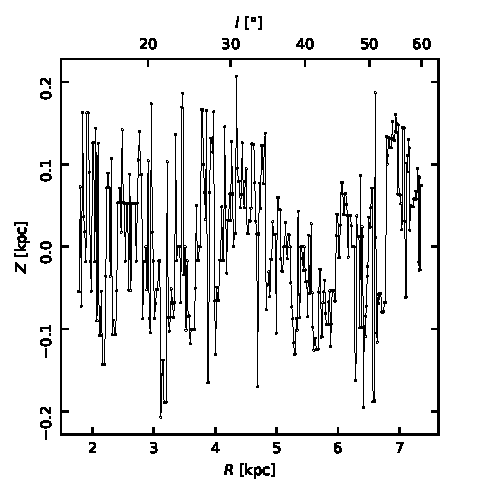
\includegraphics{rsc/Z.pdf}
	\caption{Corrugación del plano. Altura $Z$ de cada punto subcentral con respecto a la distancia galactocéntrica (eje inferior) y la longitud correspondiente (eje superior).}
	\label{fig:Z}
\end{figure}
